\documentclass{beamer}

\definecolor{Clemson}{RGB}{246,103,51}
\definecolor{ClemsonPurple}{RGB}{82,45,128}
\definecolor{myBlue}{RGB}{0,70,250}
\definecolor{myRed}{RGB}{255,0,0}
\definecolor{myYellow}{RGB}{255,255,0}
\definecolor{myPurple}{RGB}{148,0,211}
\definecolor{myOrange}{RGB}{255,140,0}
\definecolor{myGreen}{RGB}{0,100,0}
\usepackage[absolute,overlay]{textpos}
\usepackage{graphicx}
\usepackage{adjustbox}

\usepackage{bm}
\usepackage{amsthm,amsfonts}

\usepackage{tikz}
\usepackage{caption}
\usepackage{multirow}
\usepackage{subcaption}
\usetikzlibrary{shapes,arrows}

\usepackage{mathtools}
\usepackage{tikz}
\usetikzlibrary{arrows.meta,positioning}
\usepackage{pgfplots}

\newcommand{\bit}{\begin{itemize}}
\newcommand{\eit}{\end{itemize}}
\newcommand{\bem}{\begin{enumerate}}
\newcommand{\eem}{\end{enumerate}}
\mode<presentation> {
    \usetheme{Copenhagen}
    \useoutertheme{infolines}
  \useinnertheme{rounded}
  \usecolortheme[named=ClemsonPurple]{structure}
}

\usepackage[english]{babel}

\usepackage[T1]{fontenc}


\setbeamertemplate{caption}[numbered]

\setbeamertemplate{enumerate items}[default]

\title[Shorter Version of the Title]
{Actual Title}

\author[LastName1, LastName2]
{Author 1, Author 2}

\institute[Clemson]


\date[Date of Presentation]{Event Name}

\titlegraphic{
    
\includegraphics[width=3cm]{clemson-ie.png}%
    }
\subject{Talks}

\AtBeginSection[] {
  \begin{frame}<beamer>
    \frametitle{Outline}
    \tableofcontents[currentsection]
    \addtocounter{framenumber}{-1}
  \end{frame}
}

\pgfplotsset{compat=1.17}
\begin{document}

\newcommand{\exclude}[1]{}
\newcommand{\BBR}[1]{\begin{beamerboxesrounded}[scheme=wisc,shadow=true,width=0.96\textwidth]{\color{white}#1}}
\newcommand{\EBR}{\end{beamerboxesrounded}}
\beamertemplatenavigationsymbolsempty		% turn off navigation symbols

\begin{frame}
  \titlepage
\end{frame}

\begin{frame}{Slide Title}
    \begin{block}{My Theorem}
    Description of Theorem.
    \end{block}
    \bit
        \item Item 1
        \item Item 2
    \eit
    \bem
        \item Numbered item 1
        \bem
            \item Numbered item 1.1
        \eem
        \item Numbered item 2
    \eem
\end{frame}

\begin{frame}{Drawing a Network}
    \begin{center}
    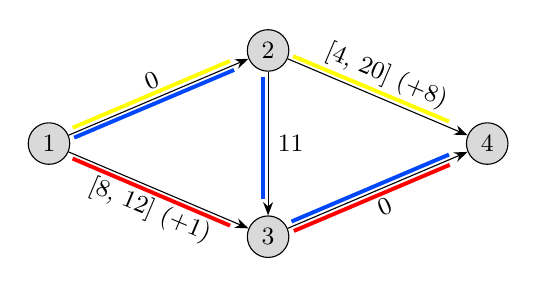
\begin{tikzpicture}[
      mycircle/.style={
         circle,
         draw=black,
         fill=gray,
         fill opacity = 0.3,
         text opacity=1,
         inner sep=0pt,
         minimum size=15pt,
         font=\small},
      myarrow/.style={-Stealth},
      node distance=0.8cm and 2.4cm
      ]
      \node[mycircle] (c1) {$1$};
      \node[mycircle,above right=of c1] (c2) {$2$};
      \node[mycircle,below right=of c1] (c3) {$3$};
      \node[mycircle,below right=of c2] (c4) {$4$};

    \foreach \i/\j/\txt/\p in {% start node/end node/text/position
      c1/c2/ 0/above,
      c1/c3/\text{[8, 12]} (+1)/below,
      c2/c4/\text{[4, 20]} (+8)/above,
      c3/c4/0 /below}
    \draw [myarrow] (\i) -- node[sloped,font=\small,\p] {\txt} (\j);
    
    \draw[->, style={-Stealth}] (c2)-- node[right,font=\small] {11} (c3);
    
    \draw[line width=0.5mm, myYellow] (0.3,0.2) -- (2.3,1.05);
    \draw[line width=0.5mm, myYellow] (3.1,1.11) -- (5.08,0.28);
    \draw[line width=0.5mm, myBlue] (0.32,0.075) -- (2.35,0.935);
    \draw[line width=0.5mm, myBlue] (2.72,0.85) -- (2.72,-0.7);
    \draw[line width=0.5mm, myBlue] (3.08,-0.99) -- (5.08,-0.14);
    \draw[line width=0.5mm, myRed] (0.3,-0.19) -- (2.3,-1.042);
    \draw[line width=0.5mm, myRed] (3.11,-1.11) -- (5.09,-0.27);
    \end{tikzpicture}
    \end{center}
\end{frame}


%%You only need the [fragile] part if you are using verbatim
\begin{frame}[fragile]{Graphs}
We can use \verb|\vspace{}| (\verb|\hspace{}|) to adjust the vertical (horizontal) position of the figure. 
\begin{figure}[tbh]\vspace*{1.0cm}\hspace*{-0.4cm}
    \centering
            \begin{subfigure}[b]{0.3\textwidth}
            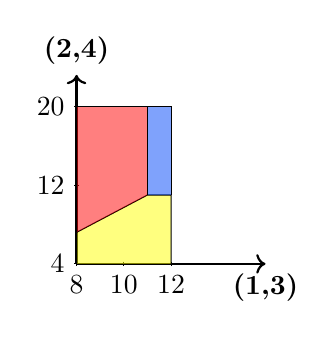
\begin{tikzpicture}[scale=0.8]
                \draw[thick,->] (0,0) -- (3,0) node[below] {\textbf{(1,3)}};
                \draw[thick,->] (0,0) -- (0,3) node[above] {\textbf{(2,4)}};
                
                \draw (0cm,1pt) -- (0cm,-1pt) node[below] {8};
                \draw (0.75cm,1pt) -- (0.75cm,-1pt) node[below] {10};
                \draw (1.5cm,1pt) -- (1.5cm,-1pt) node[below] {12};
                    
                \draw (1pt,0 cm) -- (-1pt,0cm) node[left] {4};
                \draw (1pt,1.25cm) -- (-1pt,1.25cm) node[left] {12};
                \draw (1pt,2.5cm) -- (-1pt,2.5cm) node[left] {20};
                
                \draw[fill=myYellow, fill opacity = 0.5] (0,0) -- (0,0.5) -- (1.125, 1.09375) -- (1.5, 1.09375) -- (1.5,0);
                \draw[fill=myRed, fill opacity = 0.5] (0,0.5) -- (0,2.5) -- (1.125, 2.5) -- (1.125,1.09375);
                \draw[fill=myBlue, fill opacity = 0.5] (1.125,1.09375) -- (1.125,2.5) -- (1.5,2.5) -- (1.5,1.09375);
            \end{tikzpicture}
            \vspace*{-0.8cm}\caption{Subfigure Label 1}
            \end{subfigure}
            \hfill
            \begin{subfigure}[b]{0.3\textwidth} 
            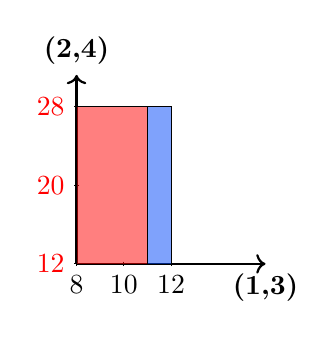
\begin{tikzpicture}[scale=0.8]
                \draw[thick,->] (0,0) -- (3,0) node[below] {\textbf{(1,3)}};
                \draw[thick,->] (0,0) -- (0,3) node[above] {\textbf{(2,4)}};
                \draw (0cm,1pt) -- (0cm,-1pt) node[below] {8};
                \draw (0.75cm,1pt) -- (0.75cm,-1pt) node[below] {10};
                \draw (1.5cm,1pt) -- (1.5cm,-1pt) node[below] {12};
                    
                \draw (1pt,0 cm) -- (-1pt,0cm) node[left] {\textcolor{red}{12}};
                \draw (1pt,1.25cm) -- (-1pt,1.25cm) node[left] {\textcolor{red}{20}};
                \draw (1pt,2.5cm) -- (-1pt,2.5cm) node[left] {\textcolor{red}{28}};
                
                \draw[fill=myRed, fill opacity = 0.5] (0,0) -- (0,2.5) -- (1.125, 2.5) -- (1.125,0);
                \draw[fill=myBlue, fill opacity = 0.5] (1.125,0) -- (1.125,2.5) -- (1.5,2.5) -- (1.5,0);
                
            \end{tikzpicture}
            \vspace*{-0.8cm}\caption{Subfigure Label 2}
            \end{subfigure}
            \hfill
            \begin{subfigure}[b]{0.3\textwidth} 
            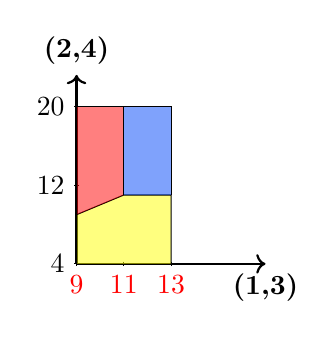
\begin{tikzpicture}[scale=0.8]
                \draw[thick,->] (0,0) -- (3,0) node[below] {\textbf{(1,3)}};
                \draw[thick,->] (0,0) -- (0,3) node[above] {\textbf{(2,4)}};
                \draw (0cm,1pt) -- (0cm,-1pt) node[below] {\textcolor{red}{9}};
                \draw (0.75cm,1pt) -- (0.75cm,-1pt) node[below] {\textcolor{red}{11}};
                \draw (1.5cm,1pt) -- (1.5cm,-1pt) node[below] {\textcolor{red}{13}};
                    
                \draw (1pt,0 cm) -- (-1pt,0cm) node[left] {4};
                \draw (1pt,1.25cm) -- (-1pt,1.25cm) node[left] {12};
                \draw (1pt,2.5cm) -- (-1pt,2.5cm) node[left] {20};
                
                \draw[fill=myYellow, fill opacity = 0.5] (0,0) -- (0,0.78125) -- (0.75, 1.09375) -- (1.5, 1.09375) -- (1.5,0);
                \draw[fill=myRed, fill opacity = 0.5] (0,0.78125) -- (0,2.5) -- (0.75, 2.5) -- (0.75,1.09375);
                \draw[fill=myBlue, fill opacity = 0.5] (0.75,1.09375) -- (0.75,2.5) -- (1.5,2.5) -- (1.5,1.09375);
            \end{tikzpicture}
            \vspace*{-0.8cm}\caption{Subfigure Label 3}
            \end{subfigure}
    \caption{Example Graph}
\end{figure}
\end{frame}

\begin{frame}{Columns}
    We can split a slide into multiple columns. 
    \begin{columns}
        \begin{column}{0.4\textwidth}
            Here is Column 1.
        \end{column}
        \begin{column}{0.6\textwidth}
            Here is Column 2.
        \end{column}
    \end{columns}
\end{frame}

\begin{frame}[fragile]{Reporting Results in a Table}
We can make the table more readable using something like \verb|\setlength{\tabcolsep}{3.5pt}|
\begin{table}
    \centering
    \setlength{\tabcolsep}{3.5pt}
    \adjustbox{scale=0.9}{%
    \begin{tabular}{rlccccclccccc}
    &  & \multicolumn{5}{c}{\textbf{Method 1}}  &   & \multicolumn{5}{c}{\textbf{Method 2}}      \\ 
    \cline{3-7}\cline{9-13}
    &  & \textit{A} & \textit{B} & \textit{C} & \textit{D} & \textit{E} & \multicolumn{1}{c}{\textit{~}} & \textit{F} & \textit{G} & \textit{H} & \textit{I} & \textit{J}  \\
    \textit{Avg} &  & 1.6         & 2.6           & 3.3          & 4.3            & 5.6           &                                & 6.3          & 7.0            & 8.9           & 9.2             & 10.2             \\
    \textit{Std} &  & 1.2         & 2.2            & 3.5           & 4.0             & 5.8           &                                & 6.7           & 7.7             & 1.6            & 0.6              & 2.2            
    \end{tabular}%
    }\caption{Here is my Caption}\label{table_1}
\end{table}
\end{frame}


\end{document}
